\subsection{Snapshot findings}
The two largest publisher contexts contain 203 and 198 selected units, respectively, and together account for 58.7\% of the frame. Eighteen of 26 contexts have fewer than five units, including 11 singleton contexts. Figure~\ref{fig:profile} shows this imbalance alongside text-length differences. The resulting archive is useful for inspecting these records but cannot supply an equal-evidence comparison of every practitioner or claimed civilization.

\begin{figure*}[!t]
\centering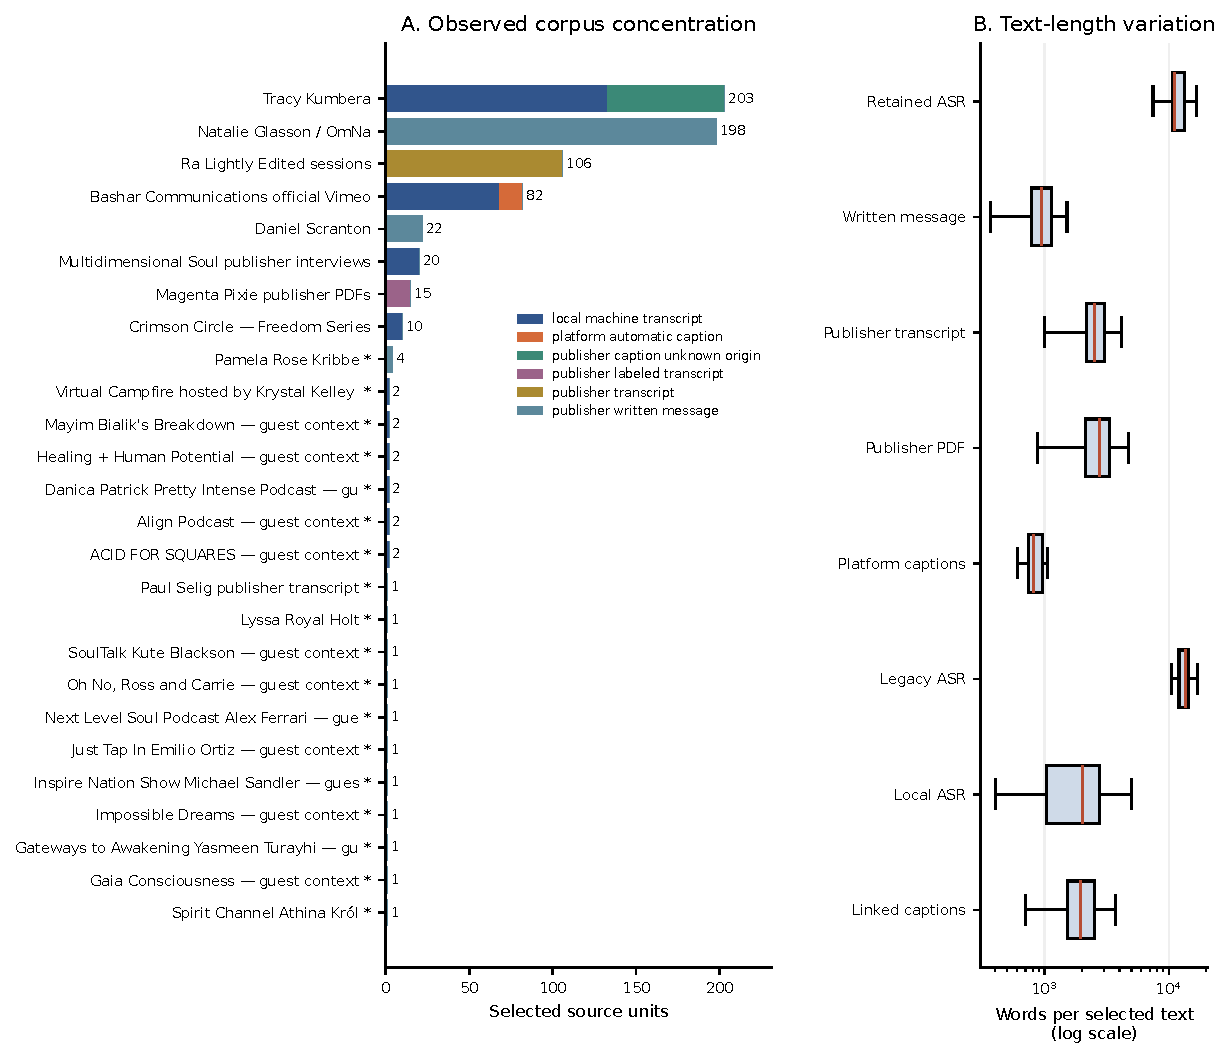
\includegraphics[width=.97\textwidth]{generated/corpus-profile.pdf}
\caption{Selected publication units by publisher context and text-length distributions. Stars mark contexts with fewer than five units. Text-origin colors are provenance categories, not quality rankings. Boxes indicate medians and interquartile ranges; whiskers extend to 1.5 interquartile ranges and outliers are not displayed. These are observed collection counts, not lifetime upload totals.}
\label{fig:profile}
\end{figure*}

The clearest diagnostic is sensitivity to the amount of text represented. Relative to masked full-text TF--IDF, the centered 300-word view has mean top-five neighbor-set Jaccard 0.137 across sources and 0.062 when contexts receive equal weight. Pairwise cosine-rank Spearman correlation is 0.536. Identity masking alone produces source-mean Jaccard 0.787; balanced-IDF fitting produces 0.782. Thus high global rank correlation under some preprocessing changes does not guarantee identical local neighbors, and the much larger length-window change cautions against treating a single similarity map as an intrinsic ordering of communications.

\begin{table}[t]
\centering\small
\begin{tabular}{lrrr}
\toprule
Contrast & $J_s$ & $J_c$ & $\rho$ \\
\midrule
Identity masking & .787 & .940 & .997 \\
Centered 300 words & .137 & .062 & .536 \\
Balanced IDF & .782 & .853 & .991 \\
Lexical vs. MiniLM (300 words) & .118 & .098 & .430 \\
\bottomrule
\end{tabular}
\caption{Top-five neighbor Jaccard averaged equally across sources ($J_s$) or publisher contexts ($J_c$), and rank correlation of pairwise similarities ($\rho$). All comparisons use the same 683-source universe. Pair scores are dependent; these values are not significance tests. The embedding comparison uses matched bounded spans, not full transcripts.}
\label{tab:sensitivity}
\end{table}

The pretrained MiniLM comparison uses the same identity-masked, centered maximum-300-word spans. Complete chunks of at most 240 content wordpieces are encoded without wordpiece truncation and pooled by content length. Its neighbor sets differ substantially from the bounded lexical representation (Table~\ref{tab:sensitivity}); this measures representation disagreement rather than an accuracy advantage. The model revision, encoder hash, and exact-input cache binding are retained. No weights were updated and no model was distilled or fine-tuned.

\begin{figure*}[!t]
\centering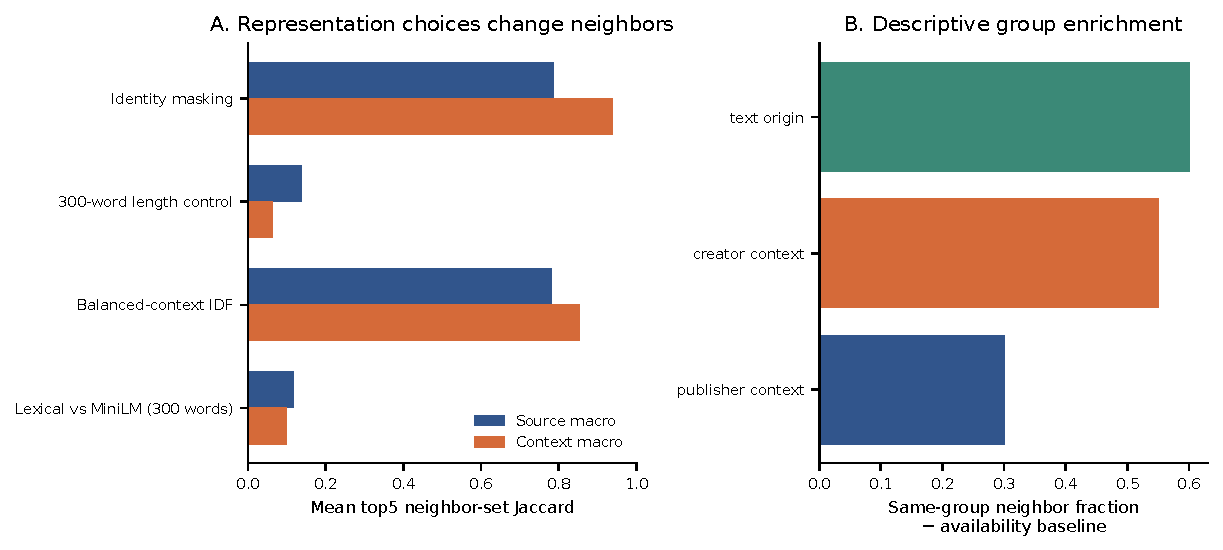
\includegraphics[width=.97\textwidth]{generated/sensitivity.pdf}
\caption{Representation sensitivity and descriptive same-group neighbor enrichment. All top-five comparisons use a common source universe. Enrichment subtracts each group's availability baseline before averaging within and equally across groups. Publisher context, creator context, text origin, and source length are confounded; these are diagnostics, not causal effect estimates.}
\label{fig:sensitivity}
\end{figure*}

NMF results are also conditional on the fit design. The eight-component main fit uses random seed 11; seeds 23 and 47 yield mean matched-component cosines 0.770 and 0.795. The mean hides heterogeneous stability: two seed-47 component matches are only 0.188 and 0.343. Their dominant-component adjusted Rand indices relative to the main fit are 0.666 and 0.737. All three runs converged under a 2,000-iteration limit, with seed 47 requiring 1,126 iterations. A separate balanced fit on 107 units has mean matched-component cosine 0.576, illustrating corpus-composition sensitivity. Figure~\ref{fig:topics} retains top-term labels, including single-letter and discourse fragments such as ``d,'' ``you're,'' and ``yeah.'' These are warnings about vocabulary and format effects, not polished evidence of doctrinal categories.

\begin{figure*}[!t]
\centering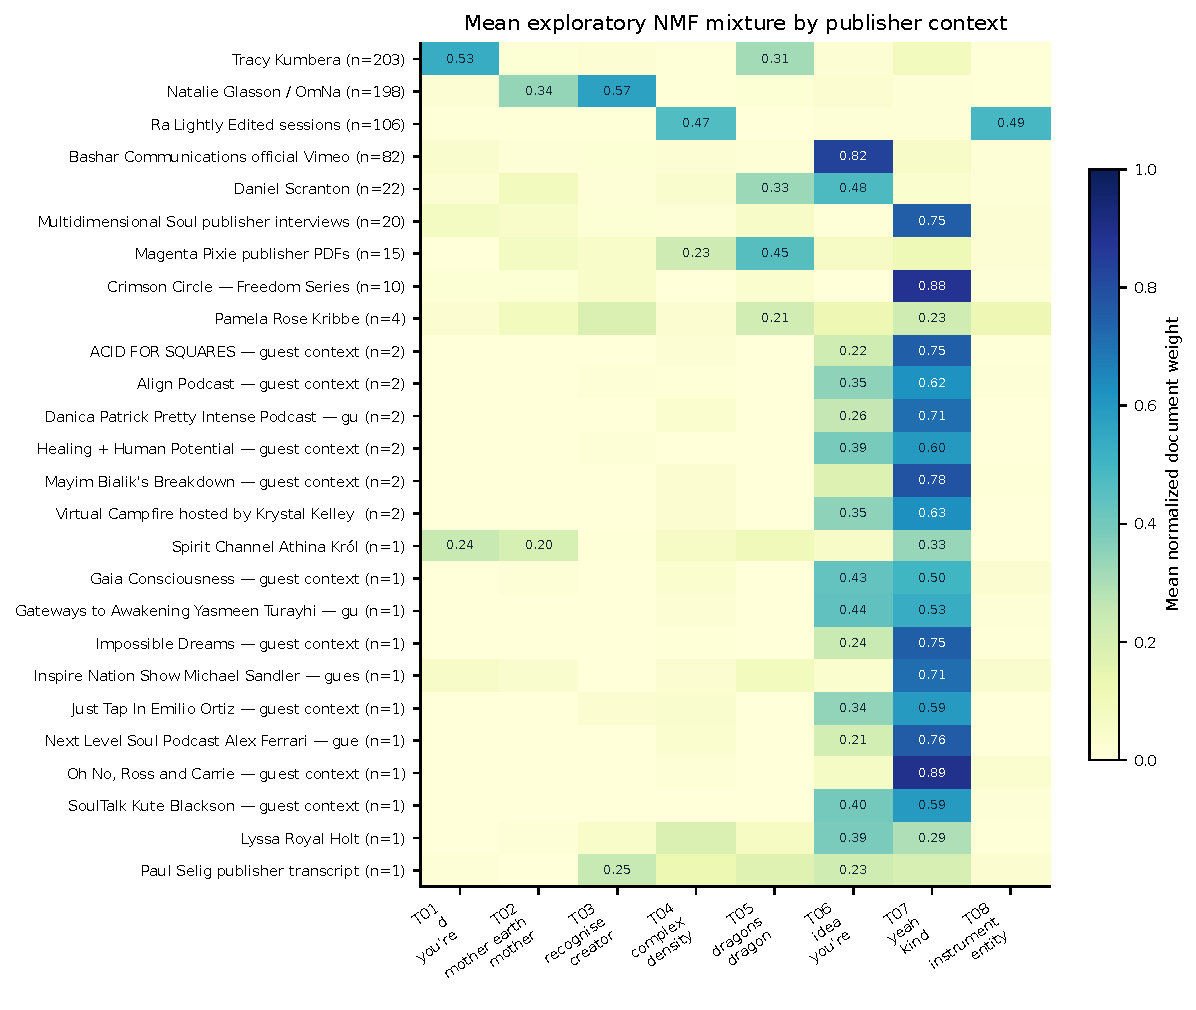
\includegraphics[width=.97\textwidth]{generated/topic-contexts.pdf}
\caption{Mean exploratory eight-component NMF mixtures by publisher context, using masked full-text TF--IDF and seed 11. Each selected source receives equal weight within its context. Labels concatenate top terms, including uninterpretable/discourse artifacts. Low-count rows and seed/composition sensitivity prevent treating these factors as a validated taxonomy.}
\label{fig:topics}
\end{figure*}

The illustrative $k=8$ clustering in normalized 50-dimensional TF--IDF SVD space has cosine silhouette 0.254 at seed 11. Its association with publisher contexts (adjusted Rand index 0.808) and text origins (0.516) underscores possible collection/format effects. Alternative values $k\in\{4,6,10\}$ and three seeds are diagnostic runs, not an optimization yielding a true number of groups. The mutual-five-neighbor graph has 888 undirected edges; these encode lexical proximity only. The two-dimensional view is lossy, and full-space cosine values remain authoritative. The exported context-similarity figure excludes self-pairs and displays contexts with at least five selected units; all 676 context cells and pair denominators remain available in exported tables. That figure, the network, and the projection diagnostics accompany the full public analysis and source ZIP.


The final analysis pass took 51.27 seconds with peak process resident memory 476,728 KiB, reusing an exact-input embedding cache. The separate original embedding pass took 63.64 seconds for 1,366 complete chunks and 245,517 content wordpieces; these are not presented as one cold-start benchmark. The code emits 9,024 punctuation-based question cues, which are explicitly unvalidated and not 9,024 observed question/answer pairs. Inspection of source passages and human transcription/annotation checks remains necessary before semantic interpretation or benchmark use.
